\section{Stokesin lause} \label{stokesin lause}
\alku
\index{Stokesin lause|vahv}

Tarkastellaan aluksi tason perusaluetta $A$ (ks.\ Luku \ref{gaussin lause}) ja $A$:ssa
määriteltyä vektorikenttää $\vec F(x,y)=F_1(x,y)\vec i + F_2(x,y)\vec j$. Kun tulkitaan $\vec F$
avaruuden vektorikentäksi, niin $\vec F$:n roottori on
(vrt.\ Luku \ref{divergenssi ja roottori})
\[
\nabla\times\vec F
    =\left(\frac{\partial F_2}{\partial x}- \frac{\partial F_1}{\partial y}\right)\vec k
    =(\text{rot}\,\vec F\,)\,\vec k,
\]
joten Greenin tasokaavojen (ks.\ Luku \ref{gaussin lause}) perusteella
\begin{align*}
\int_A \text{rot}\,\vec F\,dxdy &= \int_{\partial A} (-n_yF_1+n_xF_2)\,ds \\
&= \int_{\partial A} \vec t\cdot\vec F\,ds,
\end{align*}
missä $\vec t$ on reunan tangenttivektori suunnistettuna kuvan mukaisesti, eli $\vec t$ osoittaa
oikealle reunan ulkonormaalin suunnalta katsottuna. Tätä sanotaan reunan 
\index{positiivinen suunnistus!b@reunan}%
\kor{positiiviseksi suunnistukseksi}.
\begin{figure}[H]
\begin{center}
\import{kuvat/}{kuvapot-11.pstex_t}
\end{center}
\end{figure}
\index{kiertointegraali} \index{polkuintegraali!c@kiertointegraali}%
Integraalia yli $\partial A$:n, em. tavalla laskettuna, sanotaan \kor{kiertointegraaliksi}
ja merkitään symbolilla $\oint_{\partial A}$. Huomioiden, että
(vrt.\ Luku \ref{polkuintegraalit})
\[
\vec t\,ds=d\vec r
\] 
nähdään, että kiertointegraali on yhdistelmä polkuintegraaleja (itse asiassa työintegraaleja),
joissa kukin reunan $\partial A$ erillinen osa kierretään suunnistuksen määräämällä tavalla.
Tulos mainituin merkinnöin on siis
\begin{equation} \label{Stokesin tasokaava}
\int_A \text{rot}\,\vec F\,dxdy=\oint_{\partial A} \vec F\cdot d\vec r.
\end{equation}

Olkoon seuraavaksi $\vec F$ avaruuden vektorikenttä ja $A$ perusalue avaruustasolla $T$.
Valitaan karteesinen koordinaatisto siten, että $T$ on $xy$-taso ja kirjoitetaan tässä 
koordinaatistossa $\vec F=F_1\vec i+F_2\vec j+F_3\vec k$ ja 
$\text{rot}\vec F=\partial_x F_2-\partial_y F_1$. Tällöin nähdään, että integraalikaava 
\eqref{Stokesin tasokaava} säilyttää pätevyytensä, koska kaavassa oikealla puolella
on $d\vec r\cdot\vec k=0$, jolloin $\vec F \cdot d\vec r = (F_1\vec i+F_2\vec j) \cdot d\vec r$.
Koska kaavassa vasemmalla puolella voidaan myös kirjoittaa 
$\,\text{rot}\vec F=(\nabla\times\vec F)\cdot\vec k$, niin voidaan vetää yleisempi johtopäätös:
Jos $\vec F$ on jatkuvasti derivoituva avaruuden vektorikenttä ja $A$ on perusalue
avaruustasolla, jonka yksikkönormaalivektori on $\vec n$, niin pätee integraalikaava
\begin{equation} \label{Stokesin avaruustasokaava}
\int_A (\nabla\times\vec F)\cdot\vec n\,dS = \oint_{\partial A} \vec F\cdot d\vec r.
\end{equation}
Tässä on normaalin $\vec n$ suunta ja reunan $\partial A$ suunnistus sidottava toisiinsa siten,
että kun reunaviivaa katsellaan normaalin $\vec n$ osoittamalta puolelta, niin tilanne on kuvan
mukainen.
\begin{figure}[H]
\begin{center}
\import{kuvat/}{kuvapot-12.pstex_t}
\end{center}
\end{figure}
Kaava \eqref{Stokesin avaruustasokaava} on erikoistapaus vieläkin yleisemmästä tuloksesta,
joka tunnetaan \linebreak \kor{Stokesin\footnote[2]{\vahv{Sir George Gabriel Stokes} 
(1819-1903) oli englantilainen fyysikko--matemaatikko. \index{Stokes, G. G.|av}} lauseen}
nimellä. Stokesin lauseen mukaan kaava \eqref{Stokesin avaruustasokaava} on tietyin edellytyksin
yleistettävissä koskemaan myös avaruuden kaarevia pintoja. Tämä yleisempi tulos on
integraalikaava (Stokesin kaava)
\begin{equation} \label{Stokesin avaruuskaava}
\boxed{\quad \int_A (\nabla\times\vec F)\cdot d\vec a
                              =\oint_{\partial A} \vec F\cdot d\vec r. \quad}
\end{equation}
Tässä $\vec F$ on avaruuden vektorikenttä, $A$ on (riittävän säännöllisen muotoinen) alue
avaruuden (riittävän säännöllisellä) pinnalla $S$ ja $d\vec a=\vec n\,dS$, missä $dS$
viittaa $S$:n pinta-alamittaan ja $\vec n=$ pinnan yksikkönormaalivektori.

Kaavassa \eqref{Stokesin avaruuskaava} edellytetään, että pinnan normaali $\vec n$ ja
reunaviivan $\partial A$ suunnistus on sidottu toisiinsa edellä kuvatulla tavalla.
Tällaisen suunnistuksen järjestäminen ei ole ongelma siinä tapauksessa, että $A$ on
avaruustasolla. Avaruuden kaarevilla pinnoilla voi kuitenkin ongelmia tulla, ja yleisessä
Stokesin lauseessa pintaa $A$ onkin rajoitettava geometrisella ehdolla: Pinnan on oltava
\index{suunnistuva pinta}%
oletetulla tavalla \kor{suunnistuva}. Tarkastellaan asiaa esimerkkien valossa.

\begin{multicols}{2} \raggedcolumns
\begin{Exa} Puolipallo on suunnistuva (vrt.\ kuvio), joten Stokesin kaava
\eqref{Stokesin avaruuskaava} on sille pätevä. Kaavan voi myös todistaa pallokoordinaatteja
käyttäen: Olkoon pallo $R$-säteinen ja
\[
\vec F=F(r,\theta,\varphi)\vec e_r+F_\theta(r,\theta,\varphi)\vec e_\theta
                                  +F_\varphi(r,\theta,\varphi)\vec e_\varphi.
\]
Tällöin (vrt.\ Luku \ref{divergenssi ja roottori})
\[
\nabla\times\vec F=\frac{1}{r\sin\theta}[\partial_\theta(\sin\theta\,F_\varphi)
                  -\partial_\varphi F_\theta]\vec e_r
                  +[\ldots]\vec e_\theta+ [\ldots]\vec e_\varphi,
\]
\begin{figure}[H]
\begin{center}
\import{kuvat/}{kuvapot-13.pstex_t}
\end{center}
\end{figure}
\end{Exa}
\end{multicols}
joten kun valitaan $\vec n=\vec e_r$ (toinen vaihtoehto olisi $\vec n=-\vec e_r$), niin
\begin{align*}
\int_A (\nabla\times\vec F)\cdot d\vec a
&=\int_0^{\pi/2}\int_0^{2\pi} \frac{1}{R\sin\theta}[\partial_\theta(\sin\theta F_\varphi)
                            -\partial_\varphi F_\theta]\,R^2\sin\theta\,d\theta d\varphi \\
&= R\int_0^{2\pi}
   \left(\int_0^{\pi/2} \partial_\theta (\sin\theta F_\varphi)\,d\theta\right)d\varphi 
    -R \int_0^{\pi/2}\left(\int_0^{2\pi} \partial_\varphi F_\theta\,d\varphi\right)d\theta \\
&= R\int_0^{2\pi}\left[\sijoitus{\theta=0}
                 {\theta=\pi/2}\bigl[\sin\theta\,F_\varphi(\theta,\varphi)\bigr]\right]d\varphi
   -R\int_0^{\pi/2}\left[\sijoitus{\varphi=0}
                   {\varphi=2\pi} F_\theta(\theta,\varphi)\right]d\theta \\
&= R\int_0^{2\pi} F_\varphi(\tfrac{\pi}{2},\varphi)\,d\varphi.
\end{align*}
Reunaviivalla $\partial A$ on $\,\theta=\frac{\pi}{2}\,$ ja
$\,\vec F\cdot d\vec r=\vec F\cdot (R\,d\varphi\,\vec e_\varphi)=RF_\varphi\,d\varphi$,
joten todetaan kaava \eqref{Stokesin avaruuskaava} päteväksi puolipallolle. \loppu

%\pagebreak
\begin{Exa} Toisessa esimerkkitapauksessa tarkastellaan pintaa, joka saadaan poistamalla
suorakulmaisen särmiön ulkopinnasta kaksi vierekkäistä sivutahkoa, vrt.\ kuvio.
\begin{figure}[H]
\begin{center}
\import{kuvat/}{kuvapot-14.pstex_t}
\end{center}
\end{figure}
Tässä tapauksessa pinta koostuu tasopinnoista $A_i$, joille kullekin pätee Stokesin kaava
\eqref{Stokesin avaruuskaava}, eli
\[
\int_{A_i} (\nabla\times\vec F)\cdot d\vec a=\oint_{\partial A_i} \vec F\cdot d\vec r.
\]
Kun normaalin suunta jokaisella osalla valitaan osoittamaan särmiön ulkopuolelle, niin nähdään,
että
\begin{align*}
\int_A (\nabla\times\vec F)\cdot d\vec a 
&= \sum_{i} \int_{A_i} (\nabla\times\vec F)\cdot d\vec a \\
&= \sum_i \oint_{\partial A_i} \vec F\cdot d\vec r \\
&= \int_{\partial A} \vec F\cdot d\vec r,
\end{align*}
\begin{multicols}{2} \raggedcolumns
\parbox{5cm}{sillä viivaintegraalit osien yhteisten särmien $\partial A_i\cap\partial A_j$ yli
kumoutuvat summauksessa, vrt.\ kuvio. Siis kaava \eqref{Stokesin avaruuskaava} on
pätevä tässäkin tapauksessa. Samaan tulokseen tultaisiin myös poistamalla särmiöstä mitkä
sivutahkot tahansa (1--5 kpl). \loppu}
\begin{figure}[H]
\begin{center}
\import{kuvat/}{kuvapot-15.pstex_t}
\end{center}
\end{figure}
\end{multicols}
\end{Exa}
\begin{Exa} Kolmantena esimerkkinä tarkastellaan pintaa, joka saadaan lieriövaipasta
leikkaamalla vaippa poikki, kiertämällä toista päätä $180\aste$, ja liittämällä päät jälleen
yhteen.
\begin{figure}[H]
\begin{center}
\import{kuvat/}{kuvapot-16.pstex_t}
\end{center}
\end{figure}
%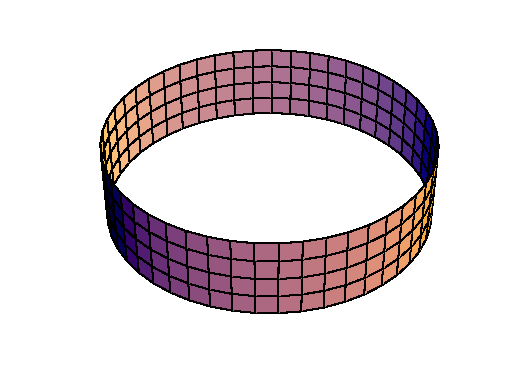
\epsfig{file=kuvat/sylvaippa.eps} $\hookrightarrow$ 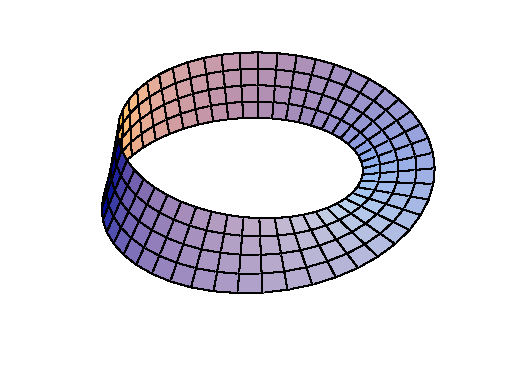
\epsfig{file=kuvat/moebius.eps}
\index{Mzz@Möbiuksen nauha}%
Tuloksena oleva pinta on nk. \kor{Möbiuksen nauha}\footnote[2]{\hist{August Möbius} (1790--1868)
oli saksalainen matemaatikko. \index{Mzz@Möbius, A.|av}}. Möbiuksen nauhalle Stokesin kaava
\eqref{Stokesin avaruuskaava} \pain{ei} ole pätevä. Sen sijaan kaava on kyllä voimassa, jos
liitossauma jätetään avoimeksi ja viivaintegraalit sauman kummallakin puolella huomioidaan
kaavassa \eqref{Stokesin avaruuskaava}. Möbiuksen nauhan tapauksessa nämä saumaintegraalit
lasketaan samansuuntaisina, jolloin ne eivät saumaa yhteen liitettäessä kumoudu, toisin kuin
lieriöpinnan tapauksessa, vrt.\ kuvio.
\begin{figure}[H]
\begin{center}
\import{kuvat/}{kuvapot-17.pstex_t}
\end{center}
\end{figure}
Möbiuksen nauha on siis erimerkki ei--suunnistuvasta pinnasta, jolle Stokesin kaava 
\eqref{Stokesin avaruuskaava} ei päde. Möbiuksen nauha on itse asiassa
\index{yksipuolinen pinta}%
\kor{yksipuolinen} pinta, jolla normaalin $\vec n$ suuntaa ei voida valita ristiriidattomasti
niin, että se muuttuisi jatkuvasti pintaa pitkin kuljettaessa.
(Jos pinta leikataan auki, niin liimauskohdassa normaali on epäjatkuva.) \loppu
\end{Exa}

Stokesin lause voidaan yksinkertaisen pinnan tapauksessa todistaa pinnan parametrisaatiota
käyttäen, mutta todistus on tällöin melko tekninen ja vaatii suhteellisen voimakkaita
säännöllisyysoletuksia. Läpinäkyvämpi ja yleispätevämpi todistus saadaan, kun pintaa
approksimoidaan kolmion muotoisilla tasopinnoilla, samalla tavoin kuin pinta-alamitan
määrittelyssä (vrt. Luku \ref{pintaintegraalit}). Koska Stokesin tasokaava pätee jokaiselle
tasokolmiopinnalle, seuraa summaamalla, että Stokesin kaava \eqref{Stokesin avaruuskaava}
pätee myös kolmioista muodostetulle pinnan $A$ approksimaatiolle --- edellyttäen, että
summauksessa viivaintegraalit yli vierekkäisten kolmioiden yhteisten sivujen kumoutuvat.
Suunnistuvuusehto on juuri tässä. Sikäli kuin pinta on suunnistuva, saadaan kolmioverkkoa
tihentämällä raja-arvotulos \eqref{Stokesin avaruuskaava} edellyttäen, että vektorikenttä
$\vec F$, pinta $A$ (pinnan parametrisaatio), ja reunaviiva $\partial A$ ovat riittävän
säännöllisiä. Vektorikentän osalta riittää, että se on jatkuvasti derivoituva
(todellisuudessa riittää hieman vähempikin), eivätkä pintaa $A$ koskevat olettamuksetkaan ole
käytännön kannalta kovin rajoittavia, vrt.\ esimerkit edellä.

Stokesin lauseella, kuten Gaussin lauseellakin, on useampiulotteiset vastineensa. Nämä kuuluvat
matematiikan alaan nimeltä \kor{differentiaaligeometria}. Tällaisiin laajempiin yhteyksiin
sijoittuu luontevimmin myös Stokesin lauseen tarkempi todistus, joka tässä sivuutetaan.
\begin{Exa}
Kappale liikkuu voimakentässä
\[
\vec F=\frac{F}{a}\,(y\,\vec i-2z\,\vec j+3x\,\vec k\,)
\]
pitkin ympyrärataa, joka on pallopinnan $x^2+y^2+z^2=a^2$ ja tason $x+y+z=0$ leikkausviiva. 
Määritä Stokesin lauseen avulla voimakentän tekemä työ yhden kierroksen aikana, kun
kiertosuunta on pisteestä $(10,10,10)$ katsottuna myötäpäivään.
\end{Exa}
\ratk Kappaleen liikerata on $\partial A$, missä $A$ on origokeskinen, $a$-säteinen kiekko
tasolla $x+y+z=0$. Stokesin lauseen mukaan
\[
W=\oint_{\partial A} \vec F\cdot d\vec r=\int_A (\nabla\times\vec F)\cdot\vec n\,dS.
\]
Tässä on
\[
\nabla\times\vec F
=\frac{F}{a} \left|\begin{array}{ccc} 
 \vec i & \vec j & \vec k \\ \partial_x & \partial_y & \partial_z \\ y & -2z & 3x
 \end{array}\right|
=\frac{F}{a}(2\vec i-3\vec j -\vec k).
\]
Oletettua kiertosuuntaa vastaa $\,\vec n=-\frac{1}{\sqrt{3}}(\vec i+\vec j+\vec k)$, joten
$(\nabla\times\vec F)\cdot\vec n = \frac{2F}{\sqrt{3}\,a}$. Siis
\[
W = \int_A \frac{2F}{\sqrt{3}\,a}\,dS = \frac{2F}{\sqrt{3}\,a}\mu(A)
  = \frac{2F}{\sqrt{3}\,a}\,\pi a^2 = \underline{\underline{(2\pi/\sqrt{3})\,Fa}}. \loppu
\]

\subsection*{Yleistetty Stokesin lause}
\index{Stokesin lause!a@yleistetty|vahv}

Kuten Gaussin lause, voidaan myös Stokesin lause yleistää niin, että pistetulon tilalla voi olla
yleisempi vektoritulo, eli joko ristitulo tai skalaarin ja vektorin kertolasku. Yleistetty
Stokesin kaava on
\[
\boxed{\quad \oint_{\partial A} d\vec r\ast\vec F=\int_A (d\vec a\times\nabla)\ast\vec F. \quad}
\]
Tässä on jälleen asetettava $\vec F\hookrightarrow f$, kun $\ast=$ `tyhjä'. Yleistetty kaava
pätee samanlaisin edellytyksin kuin peruskaava \eqref{Stokesin avaruuskaava}, ja sen voi myös 
perustella samaan tapaan kuin edellä, eli lähtemällä kaavan tasomuodosta.

\Harj
\begin{enumerate}

\item 
Olkoon $A=\{(x,y)\in \R^2 \mid x^2+y^2 \le 1\,\ja\,x \ge 0\}$. Laske seuraavat kiertointegraalit
yli $\partial A$:n (vastapäivään kiertäen) sekä suoraan viivaintegraaleina että muuntamalla ne
ensin tasointegraaleiksi (yleistettyä) Stokesin kaavaa käyttäen. \vspace{1mm}\newline
a) \ $\oint_{\partial A} \left[\,y^2\,dx+(x+y^2)\,dy\,\right] \qquad$
b) \ $\oint_{\partial A} (x+y^2)\,d\vec r$ \newline
c) \ $\oint_{\partial A} (xy^2\vec i+\abs{y}\vec j\,) \cdot d\vec r \qquad\qquad$
d) \ $\oint_{\partial_A} (y^3\vec i-x\vec j\,) \times d\vec r$

\item 
Laske $\oint_{\partial A} \vec F\cdot d\vec r$ \ a) suoraan viivaintegraalina, \  
b) Stokesin lauseen avulla, kun $\vec F=x\vec k$ ja $A \subset S$ vastaa 
parametrien arvoja $(u,v)\in [0,1]\times[0,3]$ pinnalla $\,S:\ x=8u^2,\ y=v^2,\ z=4uv$.

\item
Näytä Stokesin lauseen avulla, että jos $S$ on pallon $K:\,x^2+y^2+z^2=R^2$ ja tason 
$T:\,x+y+z=0$ leikkauskäyrä, niin $\oint_S (y\,dx+z\,dy+x\,dz)=\pm\sqrt{3}\pi R^2$.

\item
Laske pintaintegraali $\int_A \nabla\times(\vec k\times\vec r\,) \cdot d\vec a$, kun $S$, 
$A \subset S$ ja $S$:n yksikkönormaalivektorin $\vec n=n_x\vec i+n_y\vec j+n_z\vec k$
suunta on annettu seuraavilla ehdoilla. \vspace{1mm}\newline
a) \ $S:\,z=0, \quad A:\,x^2+y^2 \le 1, \quad n_z \ge 0$ \newline
b) \ $S:\,x^2+y^2+z^2=1, \quad A:\,z \ge 0, \quad n_z \ge 0$ \newline
c) \ $S:\,x^2+y^2+z^2=1, \quad A:\,z \le 0, \quad n_z \le 0$

\item
Halutaan laskea kiertointegraali $\oint_S \vec F \cdot d\vec r$ yli suljetun käyrän
$S:\,\vec r=\cos t\,\vec i+\sin t\,\vec j+\sin 2t\,\vec k,\ t\in[0,2\pi]$, kun
$\vec F=(e^x-y^3)\vec i+(e^y+x^3)\vec j+e^z\vec k$. Laske integraali Stokesin kaavan avulla
huomioimalla, että $S$ on pinnalla $z=2xy$.

\item
Olkoon $S$ lieriön $K:(x-1)^2+4y^2=16$ ja tason $T:2x+y+z=3$ \linebreak leikkauskäyrä ja
$\vec F=[\sin(x^2)+y^2+z^2]\vec i+(2xy+z)\vec j+(xz+2yz)\vec k$. Laske \linebreak
$\oint_S \vec F \cdot d\vec r$, kun $S$:n suunnistus on vastapäivään kaukaa positiiviselta
$z$-akselilta katsoen.

\item
Valitse pinnalle $A:\,z=9-x^2+y^2,\ x^2+y^2 \le 9$ suunnistus ja laske 
$\int_A \nabla\times\vec F \cdot d\vec a$, kun $\vec F=-y\vec i+x^2\vec j+z\vec k$.

\item
Laske Stokesin kaavan avulla pintaintegraali
\[
\int_{A} \nabla\times[(x-z^2)\vec i+(x^3+z)\vec j+xy\vec k] \cdot d\vec a,
\]
missä $A$ on kartiopinnan $\,S:\,x^2+y^2=(z-1)^2$ tasojen $z=0$ ja $z=1$ väliin jäävä osa.

\item 
Sähkövirran tiheys $\vec J$ ja magneettikentän voimakkuus $\vec H$ ovat lieriökoordinaatistossa
muotoa $\vec J= J(r)\vec e_z$, $\vec H = H(r)\vec e_\varphi$. Määrää $H(r)$ funktion $J(r)$ 
avulla käyttämällä Maxwellin yhtälöä $\nabla\times\vec H = \vec J$ ja Stokesin kaavaa 
sopivasti valitulla pinnalla $A$.

\item
Näytä yleistetty Stokesin kaava oikeaksi siinä tapauksessa, että $\vec F$ on avaruuden
vektorikenttä ja $A \subset T$, missä $T$ on avaruustaso.

\item
Olkoon $S$ yksinkertainen suljettu käyrä avaruustasolla $T$, jonka yksikkönormaalivektori on
$\vec n=a\vec i+b\vec j+c\vec k$. Näytä, että $S$:n sisään jäävän pinnan $A$ ala on
\[
\mu(A)=\frac{1}{2}\left|\oint_S \bigl[(bz-cy)dx+(cx-az)dy+(ay-bx)dz\bigr]\right|.
\]

\item
Määritellään pinta $A$ parametrisaatiolla
\[
A:\quad \begin{cases}
        \,x=\cos 2u(a+bv\sin nu), \\ \,y=\sin 2u(a+bv\sin nu), \\ \,z=bv\cos nu,
        \end{cases} \quad
(u,v) \in \bigl[-\tfrac{\pi}{2},\tfrac{\pi}{2}\,\bigr)\times
          \bigl[-\tfrac{\pi}{2},\tfrac{\pi}{2}\,\bigr],
\]
missä $0<b<a$ ja $n\in\N$. Millainen on $A$:n reuna $\partial A\,$? Millä $n$:n arvoilla $A$ on
suunnistuva pinta?

\item (*)
Laske kiertointegraali $\oint_S \vec F \cdot d\vec r$, kun
$\,\vec F=ye^x\vec i+(x^2+e^x)\vec j+e^z\vec k\,$ ja $S$ on suljettu parametrinen käyrä
\begin{align*}
\vec r \,=\ &(2\cos t-3\sin t)\vec i+(2+3\cos t+6\sin t)\vec j+(1+6\cos t-2\sin t)\vec k, \\
            &\,t\in[0,2\pi].
\end{align*}

\end{enumerate}